\documentclass[conference]{IEEEtran}

\usepackage[utf8]{inputenc}
\usepackage{amsmath,amssymb}
\usepackage{array}
\usepackage{booktabs,siunitx}
\usepackage{graphicx}
\usepackage{url}

\begin{document}

\title{An Enquiry into the robustness characteristics of a replaced ParaLIF vs. LIF layer on ResNet's}

\author{
    \IEEEauthorblockN{Florian Suess}
}

\maketitle

\begin{abstract}
With the work done in the main project repository\footnote{Available here; \url{https://github.com/suessflorian/biological-neurons/}} representing the findings of robustness characteristics within LIF and ParaLIF employed on networks that act on simpler datasets MNIST, KMNIST, SVHN and fashionMNIST - we find motivation to explore how these characteristics scale to much more difficult, but still locally tractable datasets such as CIFAR-10/100.
\end{abstract}

\begin{IEEEkeywords}
ResNet, ParaLIF, LIF, CIFAR-10, CIFAR-100, Advaserial Robustness, DeepFool Attack, Fast Minimum Norm MEthod, Fast Gradient Sign Method Attack, Square Attack
\end{IEEEkeywords}

\section{Introduction}
Direct training methodologies for S-NN's remain in it\'s infancy. With common approaches typically requiring backpropogation through time methods that unroll potentially an entire network linearly to the number of steps you use for a spike encoding of an input, this leads us to exceedingly longer training times per dataset. Our key biologically inspired neuron, variant of the leaky integrate and fire neuron, the "ParaLIF" addresses this facet of S-NN concern by selling us the idea that we can backpropogate through time \emph{in parallel} - but unfortunately this hasn't prevented the difficulty associated to training these networks.

One could speculate that this issue broadly steps parallel to issues faced by the training of traditional recurrent networks, albeit in the case of S-NN's, we face these issues without the mechanisms such as the LSTM and GRU gradient preserving gates. It is left to the reader to devise a study on gradient flows through these style networks and issue findings. We instead sprint to alternative training methods to more quickly see the scaling of these robustness characteristics.

\section{Alternative Training Methods}
We have previously in our journey to break our performance boundaries found ANN-SNN conversions effective\footnote{Available here; https://github.com/suessflorian/qcfs/}. We specifically adapted methods published in the literature specific to ResNets. This involved priming techniques (concretely, that is, swapping all ReLU's with "quantised clip-floor shifted" ReLU) such that a recursive activation swap with LIF had a zero conversion error loss. However we deemed this method a bit too restrictive to continue with - predominately because a mapping to ParaLIF activation functions was unclear, placing a very resource intensive challenge to breakthrough. With the little time we had we had, we picked out what worked well, simplified the problem that served our original research question.

\section{Simplifying to Hybrid Models}
As already seen earlier, a large concession we made early on was to step away from \emph{pure S-NN's} which are defined as; a network that propagates forward in discrete values. This style of S-NN has specifically been rocking the label "the third-generation of neural networks" since the late 90's and is becoming even more relevant due to their unique plausibility to run on neuromorphic hardware; specialized event-driven hardware reduced to represent signals through sparse, asynchronous spikes offering substantial efficiency in both energy consumption and computational speed (no need for a sync clock).

Although we value this more broadly, and some of us hope to continue in this research area, our specific focus lives within the adversarial robustness characteristics of LIF and ParaLIF activations. With the introduction of convolutions into our networks, we can leverage their known performance characteristics on image classification tasks.

\section{Looking at ResNet Models}
The key idea here is to use a ResNets as an encoder of our input up to the point of exit from the 4th residual layer, decoding this feature map using a single ParaLIF/LIF feed forward linear layer. We batch min max normalise the feature map values into the range $p \in [0,1]$. We use this to "rate encode" this over 20 steps using the same Bernoulli distribution method used throughout this research project. Each step assuming 1 with probability $p$ and 0 with probability 1-$p$. We semi-arbitrarily choose the ResNet models 18 and 50 due to their ubiquitous names for benchmarking model performance progresses recently.

\subsection{Transfer Learning}
We adopt what we learnt in the QCFS ANN-SNN endeavour and focus on conversion tactics. We train the respective ResNets unchanged. Leveraging the speed up boost by transferring pre-trained weights from heavily trained ResNets on the ImageNet. At the time of this enquiry, we had some readily available (and verifiable) performance characteristics of the following;

\vspace{0.5cm}
\begin{table}[ht]
\centering
\begin{tabular}{ l l l }
  \toprule
  Model & \multicolumn{1}{c}{Accuracy \%} & \multicolumn{1}{c}{Parameters (M)} \\
  \midrule
  ResNet-18 & \num{69.76} & \num{11.7} \\
  ResNet-50 & \num{80.86} & \num{25.6} \\
  \bottomrule
\end{tabular}
\end{table}

\pagebreak

Unfortunately, even with these pre-trained weights available to us - ImageNet is still intractable given the compute we had available to us so we felt the need to simplify datasets to CIFAR-100 and CIFAR-10. This required a fine-tuning phase of these existing models. Training the full network is prone to destructive learning, especially to those low level feature layers - and so we experimented with freezing early residual layers, found that freezing all parameters pre layer 3 was effective.

We didn't have too much time to experiment much with all the various available meta learning hyper parameters but we found the classic SGD optimization method was sufficient, with a low $\alpha=0.001$, basic L2 weight regularisation with some training speed increases too with introduced momentum during descent.

We found more training speed gains by stabilising the 4th residual layer using the default ResNet configuration before transferring to ParaLIF and LIF activations - and so we have indeed demonstrated a \emph{double} learning transfer approach to this issue of limited compute.

\section{Test Performance Measure}
\begin{figure}[h!]
    \centering
    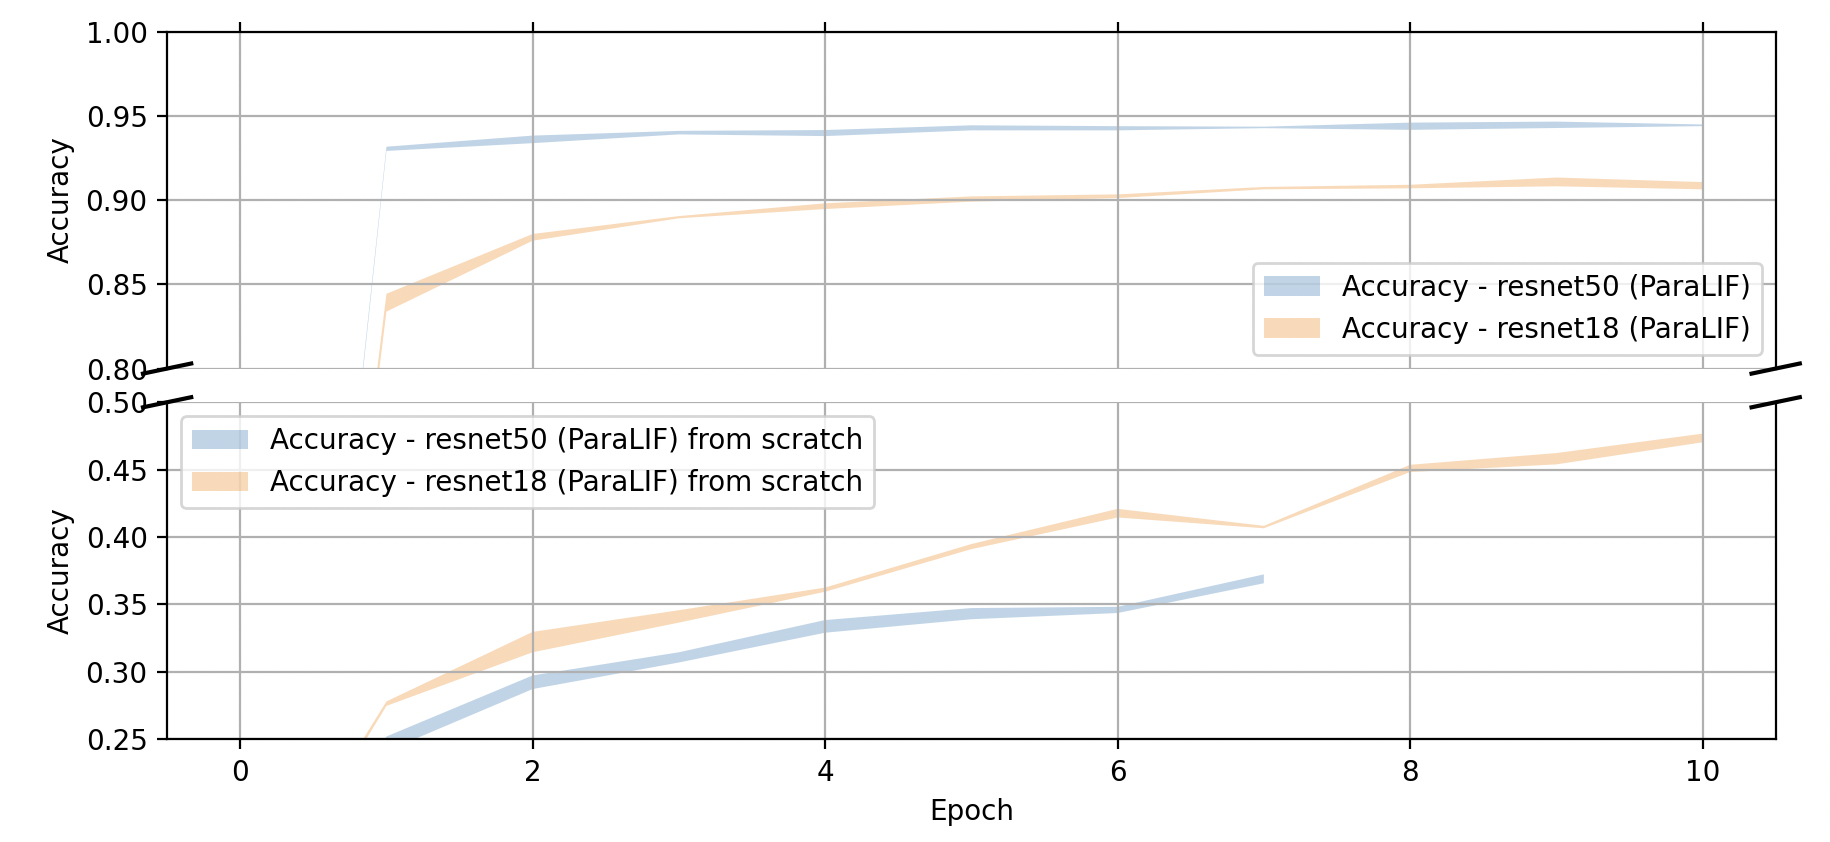
\includegraphics[width=\linewidth]{transfer-contrast.png}
    \caption{The double transfer method test accuracy climbing quickly relative to scratch training}
    \label{fig:transfer_contrast}
\end{figure}

With all of this careful planning, on execution - we quickly surpass previous model performance by significant margin. Allowing for deeper enquiry into CIFAR-10 with a comfortable dataset beat allowing us to start paying attention to CIFAR-100. Although both LIF and ParaLIF contain a stochastic element in their inference (the Bernoulli distribution rate encoding method), we found notable variance in inference outcomes given a fixed image on different random seeds - hence we accompany test results with standard deviation.



\begin{itemize}
    \item All default variants are trained for 10 epochs.
    \item ParaLIF/LIF variants are trained for 10 epochs, with transferred weights of a fine-tuned 4th residual layer from the above.
\end{itemize}

\begin{table}[ht]
\centering
\begin{tabular}{ l l l }
  FashionMNIST \\
  \\
  Variant & \multicolumn{1}{c}{ResNet-18} & \multicolumn{1}{c}{ResNet-50} \\
  \midrule
  Default & \num{93.2} & \num{93.2} \\
  LIF & \num{93.7} & \num{93.4} \\
  ParaLIF & $91.5\% \pm 0.08\%$ & $92.5\% \pm 0.14\%$ \\
  \bottomrule
\end{tabular}
\end{table}

\begin{table}[ht]
\centering
\begin{tabular}{ l l l }
  CIFAR-10 \\
  \\
  Variant & \multicolumn{1}{c}{ResNet-18\%} & \multicolumn{1}{c}{ResNet-50} \\
  \midrule
  Default & \num{92.4} & \num{94.7} \\
  LIF & \num{92.8} & \num{94.8} \\
  ParaLIF & $90.9\% \pm 0.15\%$ & $94.4\% \pm 0.034\%$ \\
  \bottomrule
\end{tabular}
\end{table}

\begin{table}[ht]
\centering
\begin{tabular}{ l l l }
  CIFAR-100 \\
  \\
  Variant & \multicolumn{1}{c}{ResNet-18 \%} & \multicolumn{1}{c}{ResNet-50} \\
  \midrule
  Default & \num{73.3} & \num{77.9} \\
  LIF & \num{74.3} & \num{79.4} \\
  ParaLIF & $34.9\% \pm 0.08\%$ & $52.9\% \pm 0.14\%$ \\
  \bottomrule
\end{tabular}
\end{table}

\section{Attacks}
We proceed from here to start attacking these models with the following attacks;

\begin{itemize}
    \item Whitebox
        \subitem Fast Gradient Sign Method Attack (FGSM)
        \subitem Fast Minimum Norm Method (FMIN)
        \subitem DeepFool Attack

    \item Blackbox
        \subitem Square Attack

With each method, we are interested in contrastive performance wrt. each dataset and model. To gauge how comparable these attacks are with respect to perturbation severities we supplement our results here with relative SSIM measures between the adversarial image built by the attack and the original image. Accompanying also is standard deviations for the ParaLIF model due it's noticeable inference instability.

\subsection*{Fast Gradient Sign Method Attack}
\subsection*{Fast Minimum Norm Method Attack}
\subsection*{DeepFool Attack}
\subsection*{Square Attack}
\begin{figure}[h!]
    \centering
    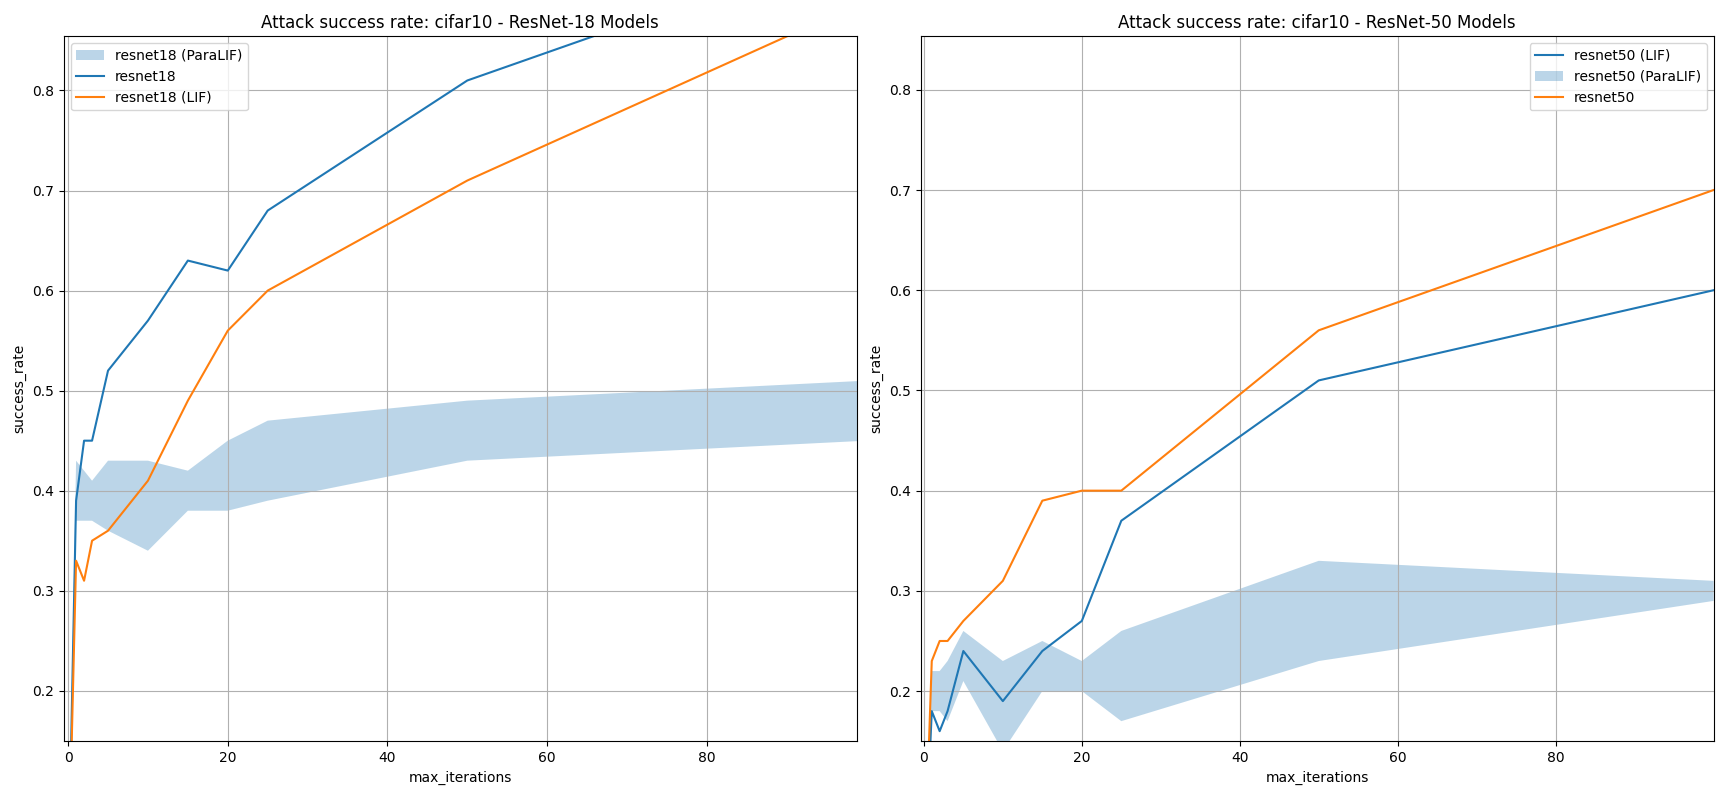
\includegraphics[width=\linewidth]{square-cifar10.png}
    \caption{Square attack at a fixed $\epsilon=0.1$ at various max attack iterations}
    \label{fig:square_attack}
\end{figure}


\end{itemize}

\end{document}
